\documentclass[10pt]{beamer}
%\usetheme{Boadilla}
%\usecolortheme{beaver}
%\usepackage[latin1]{inputenc}
\useoutertheme{split}
\setbeamertemplate{navigation symbols}{}
\usefonttheme[onlymath]{serif}
\usepackage{amsmath}%
\usepackage{amsthm}%
\usepackage{amsfonts}%
\usepackage{amssymb}%
\usepackage[algo2e]{algorithm2e}
\usepackage{algorithmic}  
\usepackage{algorithm}
\usepackage{tikz}
\usepackage[english]{babel}
\usepackage{amsmath, amssymb, amsthm}
\usepackage{verbatim}
\usepackage{mathrsfs}
%\usepackage{epstopdf}
\usepackage{graphicx}
\mode<presentation>
{
	\usetheme{CambridgeUS}
	\usecolortheme{dolphin}
	\usecolortheme{rose}
	\setbeamercovered{transparent}
}
\newcommand{\mrel}{\mathrel{\bigcirc}}
%\usepackage[onehalfspacing]{setspace}
%\setbeamertemplate{footline}[frame number]
\DeclareMathOperator*{\Bigcdot}{\scalerel*{\cdot}{\bigodot}}
% Macros
\def\a{\alpha} \def\b{\beta} \def\c{\gamma} \def\d{\delta} \def\r{\rho}
\def\e{\epsilon} \def\ve{\varebsilon} \def\k{\kappa} \def\p{\pi} \def\th{\theta}
\def\l{\lambda} \def\m{\mu} \def\s{\sigma} \def\t{\tau} \def\w{\omega} \def\z{\zeta}
\def\D{\Delta} \def\G{\Gamma} \def\W{\Omega} \def\P{\Phi} \def\L{\Lambda}
\def\bdm{\begin{displaymath}} \def\edm{\end{displaymath}}
\def\bni{\begin{itemize}} \def\ei{\end{itemize}}
\def\bnen{\begin{enumerate}} \def\een{\end{enumerate}}
\def\fa{\forall}
\def\be{\begin{equation}} \def\ee{\end{equation}}
\def\fn{\footnote} \def\bn{\begin} \def\nit{\noindent}
\def\iff{\textit{~if and only if~~}}
\renewcommand*{\thefootnote}{\fnsymbol{footnote}}
% THEOREMS -------------------------------------------------------
\newtheorem{thm}{Theorem}%[section]
\newtheorem{cor}[thm]{Corollary}
\newtheorem{lem}[thm]{Lemma}
\newtheorem{prop}[thm]{Proposition}
\newtheorem{claim}{Claim}
\theoremstyle{definition}
%\newtheorem{defn}[thm]{Definition}
\theoremstyle{remark}
\newtheorem{rem}[thm]{Remark}
%%\numberwithin{equation}{section}  
 
\newcommand{\N}{\mathbb{N}}
\newcommand{\Z}{\mathbb{Z}}
\newcommand{\R}{\mathbb{R}}
\newcommand{\ls}{\left\{}
\newcommand{\rs}{\right\}}


\title[Interaction-Partitioned Topic Model (IPTM)]{ \vspace{-.25cm} \\ A Network Model for \\Dynamic Textual Communications \\with Application to
	Government Email Corpora}
\author[\quad B. Kim, A. Schein, B. Desmarais and H. Wallach\quad]{
Bomin Kim\textsuperscript{1}\and
\quad Aaron Schein\textsuperscript{3}\and\\
		Bruce Desmarais \textsuperscript{1}\and Hanna Wallach\textsuperscript{2,3}}
\institute{\textsuperscript{1} The Pennsylvania State University \and \textsuperscript{2} Microsoft Research NYC \and \textsuperscript{3} University of Massachusetts Amherst}


\begin{document}
 
\begin{frame}
  \titlepage
  \begin{center}
   \begin{tabular}{cc}
\hspace*{-.2in} \tiny \begin{minipage}{3.5in}
Work supported by NSF grants SES-1558661, SES-1619644, SES-1637089, and CISE-1320219)\\ ~\\~\\~\\~\\
\end{minipage}
& \includegraphics[scale=.05]{figures/NSF_logo.png}
\end{tabular}
\end{center}
\end{frame}




\begin{frame}{Motivation}
\Large
\begin{itemize}
\item In many networks, ties are attributed with text
\begin{itemize}
\item International treaties
\item International sanctions
\item Legislative cosponsorship
\item Discussion networks on social media
\end{itemize}
\vspace{.2cm}
\item Network models can't model text
\vspace{.3cm}
\item Models for text either...
\begin{itemize}
\item Are not designed for networks
\item Include simplistic network structure
\end{itemize}
\end{itemize}
\end{frame}

\begin{frame}{Interaction-Partitioned Topic Model (IPTM)}
\large
	\bni
	\item Probablistic model for time-stamped textual communications \\
	\vspace{0.2cm}
	\item Integration of two generative models:\\
		\vspace{0.1cm}
	 - Latent Dirichlet allocation (LDA) for topic-based contents\\	\vspace{0.2cm}
	 - Dynamic exponential random graph model (ERGM) for ties \\
	\ei
		\vspace{0.4cm}
\centering \large\textit{``who communicates with whom about what, and when?"}
\end{frame}

\begin{frame}{Content Generating Process: LDA (Blei et al., 2003)}
\bni 
\begin{minipage}{0.7\linewidth}
\item For each topic $k =1,...,K:$\vspace{0.2cm}
	\begin{itemize}
		\item[1.] Choose a topic-word distribution over the word types\vspace{0.2cm}
		\item[2.] Choose a topic-interaction pattern assignment			
		\end{itemize}
		\vspace{0.2cm}
	\end{minipage}
	\begin{minipage}{0.25\linewidth}
			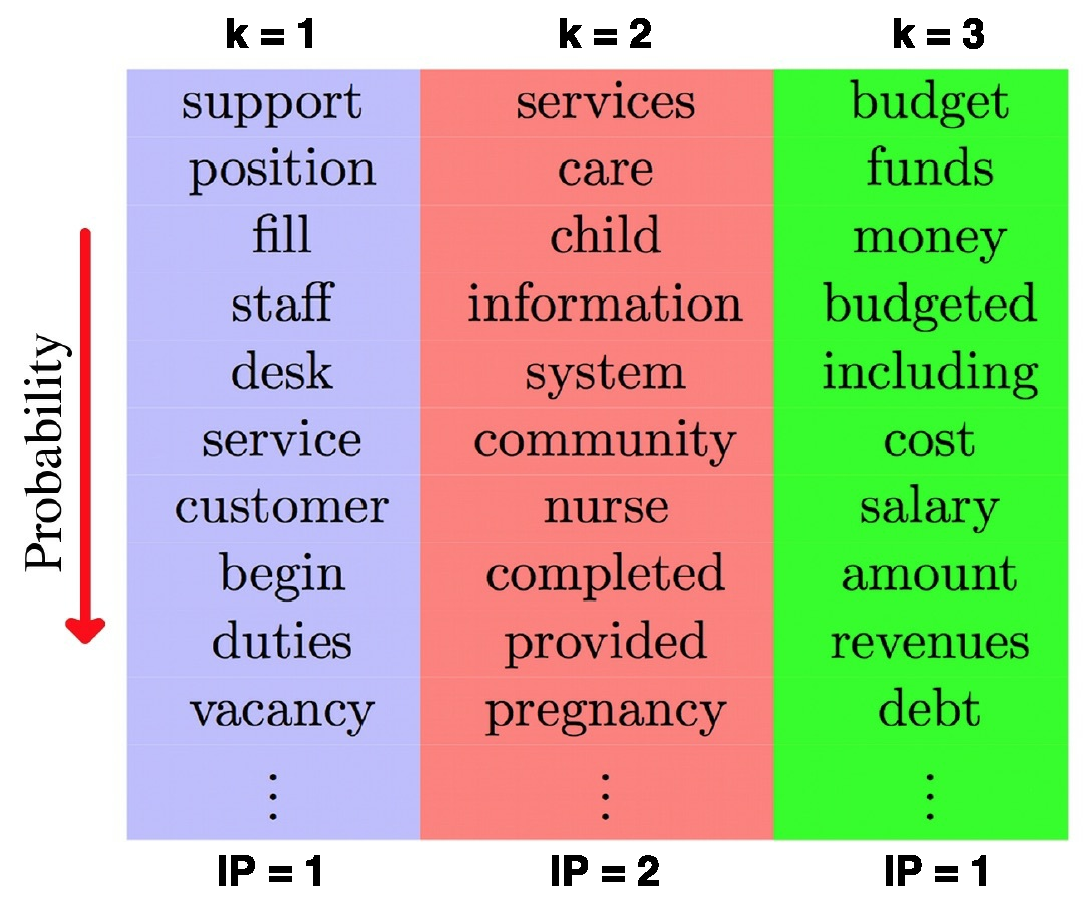
\includegraphics[width=1\textwidth]{figures/word.pdf}
				\vspace{0.2cm}
		\end{minipage}
			\begin{minipage}{0.68\linewidth}
				\item For each document $d =1,...,D:$ \vspace{0.2cm}
		\begin{itemize}
					\item[3-1.] Choose a document-topic distribution \\\vspace{0.1cm} 
		\item[3-2.] For each word in a document $n=1$ to $N^{(d)}$:\vspace{0.1cm} 
		\begin{itemize}
			\item[(a)] Choose a topic from document-topic distribution\vspace{0.2cm} 
			\item[(b)] Choose a word from topic-word distribution
		\end{itemize} 
			\end{itemize}
		\end{minipage}
		\begin{minipage}{0.3\linewidth}
	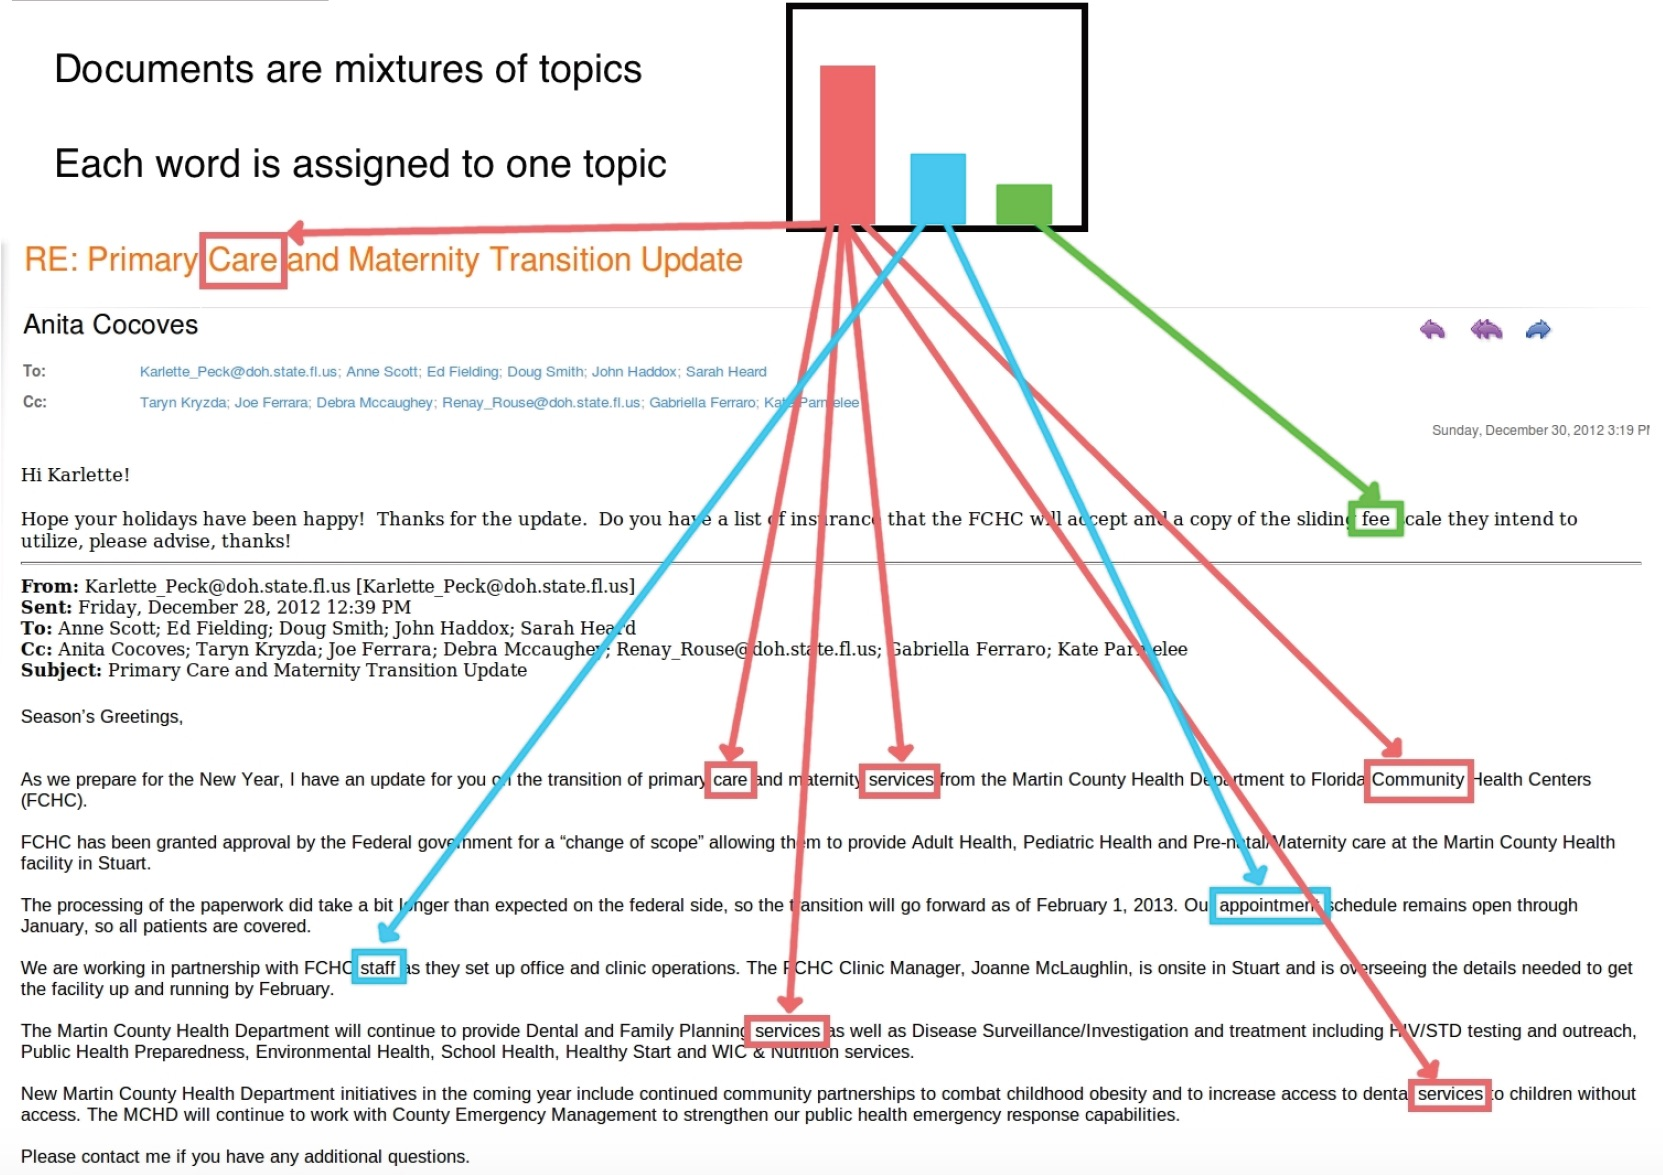
\includegraphics[width=1.05\textwidth]{figures/LDAimage.jpeg}
		\end{minipage}
		\vspace{0.2cm}
				\begin{itemize}\item[3-3] Calculate the distribution of interaction patterns within a document:
		 \footnotesize\begin{equation*}
		p_c^{(d)} = \Big({\sum\limits_{k: c_k=c} N^{(k|d)}}\Big)/{N^{(d)}},
		\end{equation*}\normalsize
	\end{itemize}
\ei	
\end{frame}


\begin{frame}{Network Model Components}
\large
\begin{itemize}
\item Models real time ties \vspace{.2cm}
\item Ties predicted using recent network structure 
\begin{itemize}
\item Vertex attributes
\item Popularity
\item Reciprocity
\item Transitivity
\end{itemize} \vspace{.1cm}
\item Sender selects vector of recipients and timing \vspace{.2cm}
\item Innovative modeling of multicasts
\end{itemize}


\end{frame}

\begin{frame}{Dynamic Network Features (Perry and Wolfe, 2012)}

\large
Current network features modeled
\begin{itemize}
\item memory
\item reciprocity
\item popularity and activity
\item transitivity
\end{itemize}

	 \begin{figure}
	 	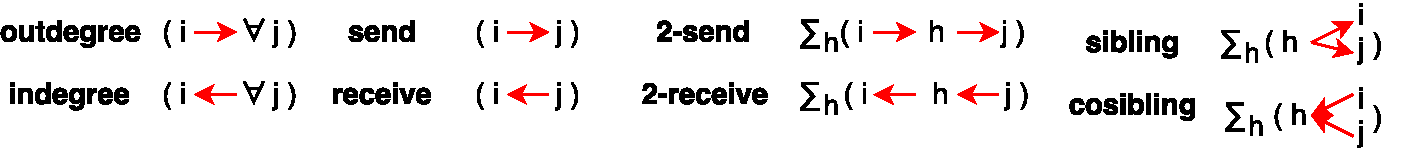
\includegraphics[height= 2cm, trim= 0cm 0cm 14cm 0cm, clip=true]{figures/netstats.pdf}\\ \vspace{-.5cm}
		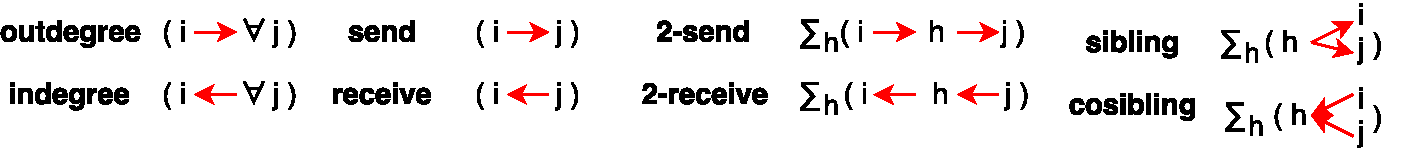
\includegraphics[height= 2cm,, trim= 10cm 0cm 0cm 0cm, clip=true]{figures/netstats.pdf}
	 \end{figure}	

\end{frame}

\begin{frame}{Conditioning feagures on recency}


\begin{itemize}
\item Network features conditioned on degree of recency
\item Partition the past 384 hours (=16 days) into 3 sub-intervals
	\begin{equation*}
	[t-384h,t) = [t-384h, t-96h) \cup [t-96h, t-24h)\cup [t-24h, t),
	\end{equation*}
\item $\boldsymbol{x}^{(c)}_{t, l}(i, j)$ is the network statistics at time $t$, for interaction pattern $c$
\end{itemize}
\centering
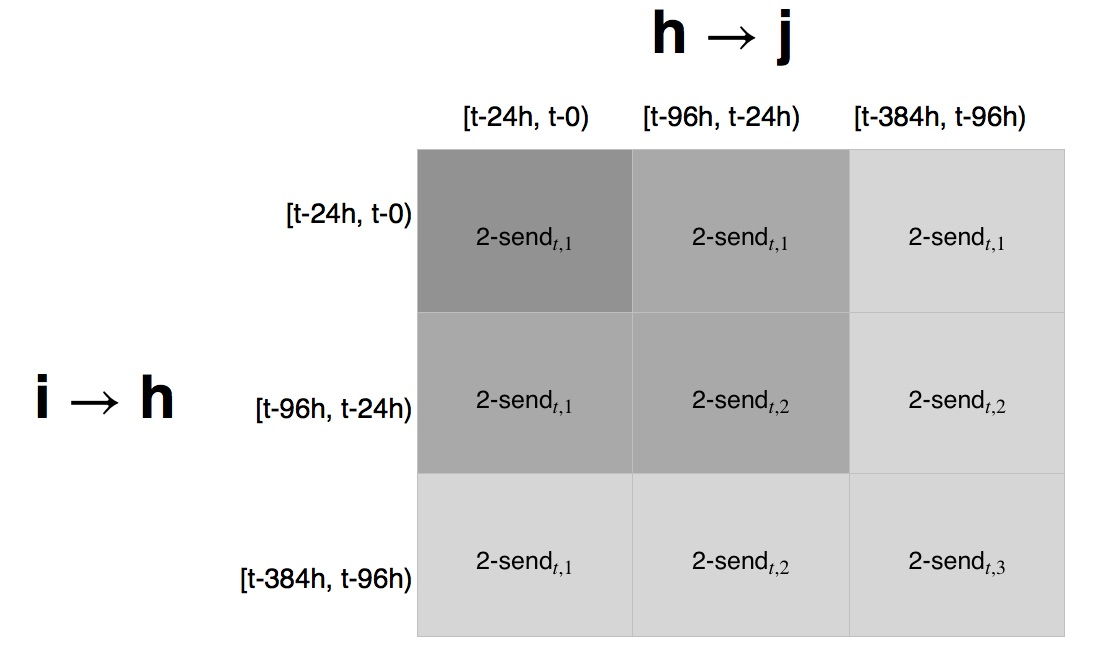
\includegraphics[scale=.2]{./figures/triadtable}

\end{frame}

\begin{frame}{Tie Generating Process: Receivers}
		\begin{itemize}
		\item [1.] For each sender $i \in \{1,...,A\}$ and receiver $j \in \{1,...,A\}$ ($i \neq j$), calculate the stochastic indensity between $i$ and $j$:
	%	\footnotesize
			\begin{equation*}\lambda^{(d)}_{ij}=\sum\limits_{c=1}^{C} p^{(d)}_c
		\cdot  \mbox{exp}\Big\{\boldsymbol{b}^{(c)}_0 + \boldsymbol{b}^{(c)T}\boldsymbol{x}^{(c)}_{t^{(d-1)}}(i, j)\Big\},	\end{equation*}\normalsize
		which is a mixture of contents, baseline interaction rate, and network effects.\\ \vspace{0.4cm}
		\item[2.] For each sender $i \in \{1,...,A\}$, choose a binary vector $J^{(d)}_i$ of length $(A-1)$, by applying Gibbs measure (Fellows and Handcock, 2017) 
	%	\footnotesize
		%\mbox{log}\big(\text{I}( \sum_{j \in \mathcal{A}_{\backslash i}} J^{(d)}_{ij} > 0 )\big) + 
		\begin{equation*} \text{P}(J_i^{(d)}) \propto \exp\Big\{ \sum_{j \in \mathcal{A}_{\backslash i}} (\delta+\mbox{log}(\lambda_{ij}^{(d)}))J_{ij}^{(d)} \Big\},
		\end{equation*}
		\normalsize
		where $\delta$ is a real-valued intercept controlling the recipient size\\ \vspace{0.1cm}
 \begin{figure}
 	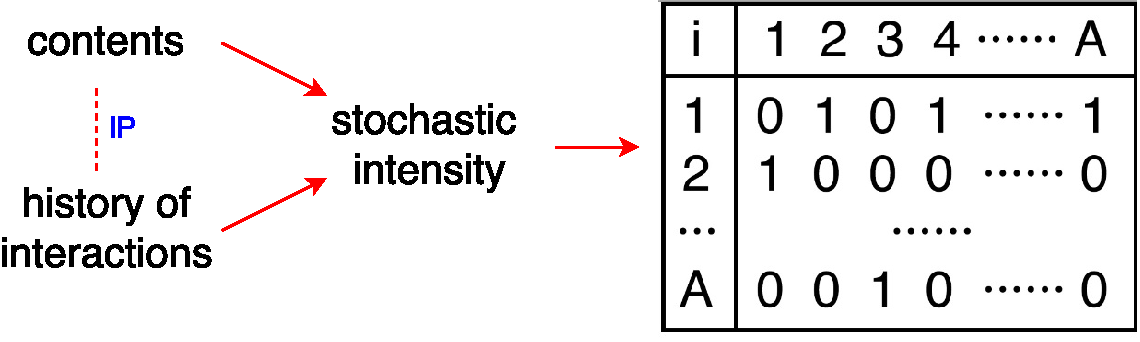
\includegraphics[width=0.4\textwidth]{figures/edge.pdf}
 \end{figure}	
	\end{itemize}
	\end{frame}
\begin{frame}{Tie Generating Process: Sender and Time}
\begin{itemize}
		\item [3.] For each sender $i \in \{1,...,A\}$, generate the time increments for document $d$
	%	\footnotesize
		\begin{equation*}
		\Delta T^{(d)}_{i{J_i}} \sim \mbox{Exponential}(\lambda_{i{J_i}}^{(d)}),
		\end{equation*}\normalsize
		where \footnotesize$\lambda^{(d)}_{iJ_i}= \sum\limits_{c=1}^{C} p^{(d)}_c\cdot\mbox{exp}\Big\{\lambda^{(c)}_0+\textcolor{gray}{\frac{1}{|J_i|}\sum\limits_{j \in J_i} \boldsymbol{b}^{(c)T}\boldsymbol{x}^{(c)}_{t^{(d-1)}}(i, j)}\Big\}\quad$\normalsize is the updated sender-specific stochastic intensity given the receivers.\vspace{0.4cm}
		\item[4.] Set the observed sender, receivers and timestamp simultaneously:
		%\footnotesize
			\begin{equation*}
		\begin{aligned}
		&i^{(d)} = i_{\mbox{min}(\Delta T^{(d)}_{i{J_i}})} \\
		&J^{(d)} = J_{i^{(d)}}\\
		&t^{(d)} = t^{(d-1)}+\mbox{min}(\Delta T^{(d)}_{i{J_i}})\\
		\end{aligned}
		\end{equation*}
		\normalsize
\end{itemize}
 %\begin{figure}
 %	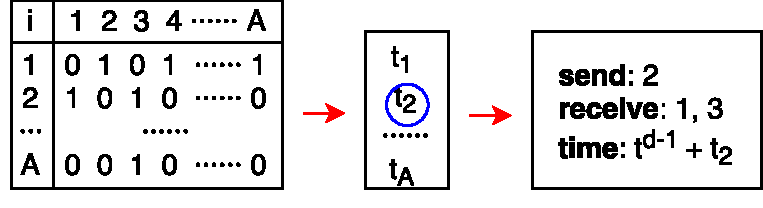
\includegraphics[width=0.57\textwidth]{figures/tie.pdf}
 %\end{figure}	
\end{frame}

\begin{frame}{Joint Generating Process}

	\begin{figure}
		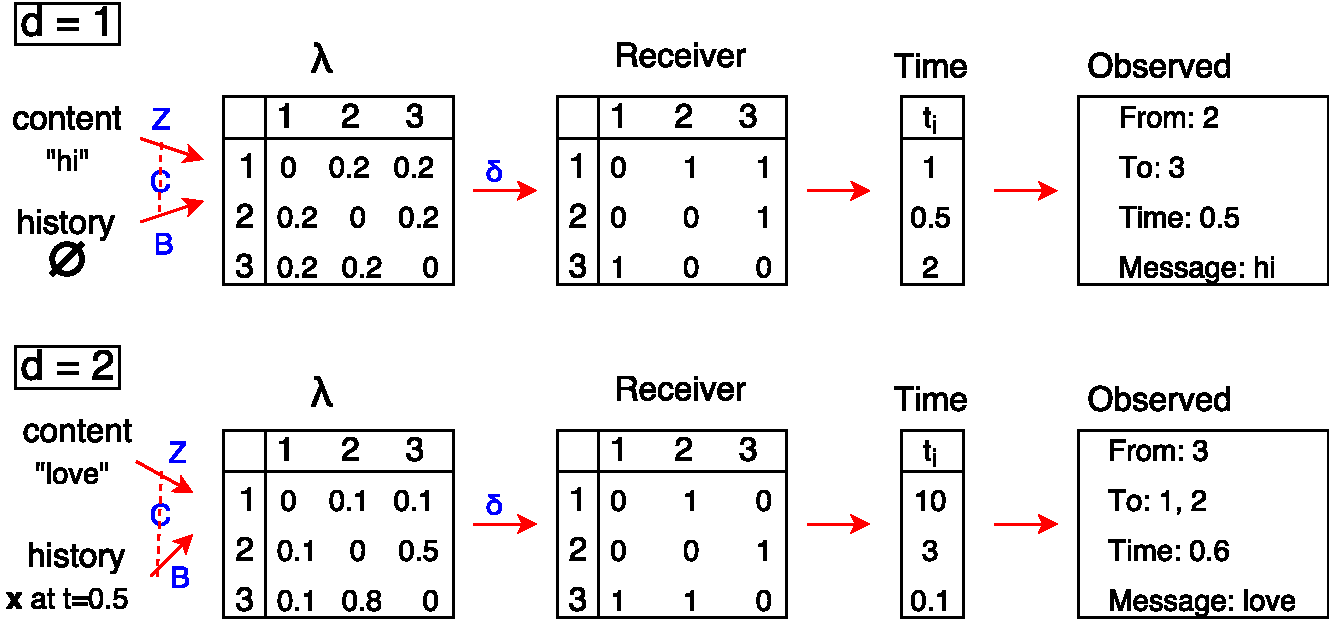
\includegraphics[width=0.9\textwidth]{figures/summary.pdf}
	\end{figure}	\vspace{0.1cm}

\end{frame}


\begin{frame}{Inference}

\begin{itemize}
\item Take a Bayesian approach to inference
\item $\mathcal{B}$ and $\delta$ interpreted at fixed $\mathcal{Z}$ and  $\mathcal{C}$
\end{itemize}
  	\begin{center}
  		\scalebox{.9}{	 
 	 \begin{minipage}{1\linewidth}\begin{algorithm}[H]
\SetAlgoLined
	 	\caption{MCMC}
	 	Set initial values $\mathcal{Z}^{(0)}, \mathcal{C}^{(0)}, $ and $(\mathcal{B}^{(0)}, \delta^{(0)})$\\
	 	\For{o=1 to O}{
	 				Sample the \textcolor{blue}{latent receivers} $J^{(d)}_{ij}$ via Gibbs sampling\\
	 				Sample the \textcolor{blue}{topic assignments} $\mathcal{Z}$ via Gibbs sampling\\
	 			Sample the \textcolor{blue}{interaction pattern assignments} $\mathcal{C}$ via Gibbs sampling\\
	 		 				Sample the \textcolor{blue}{network effect parameters} $\mathcal{B}$  via Metropolis-Hastings \\
	 			Sample the \textcolor{blue}{receiver size parameter} $\delta$ via Metropolis-Hastings
	 	}
	 \end{algorithm}
	\end{minipage}}
	 	\end{center}
\end{frame}


\begin{frame} \frametitle{Getting it Right: Jointly testing math and code}

Geweke (2004) proposed a test for Bayesian posterior samplers \vspace{.2cm}
\begin{itemize}
\item {\em Forward samples}: 
\begin{enumerate}
\item Draw parameters from prior
\item Draw data conditional on parameters
\item Repeat
\end{enumerate} \vspace{.2cm}
\item {\em Backward samples}: 
\begin{enumerate}
\item Start with a forward sample of data
\item Run inference on data
\item Generate new data conditioned on inferred parameters
\item Run inference on new data
\item Repeat
\end{enumerate} \vspace{.2cm}
\item Forward samples and backward samples should match
\end{itemize}


\end{frame}

\begin{frame} \frametitle{GiR: Results with full model}
\centering \vspace{-.4cm}
\includegraphics[scale=.485]{./figures/Schein_C_50k.pdf}

\end{frame}

\begin{frame} \frametitle{GiR: Results with fixed C}
\centering \vspace{-.4cm}
\includegraphics[scale=.485]{./figures/Schein_noC_50k.pdf}

\end{frame}


\begin{frame}{North Carolina county email data}
 \bni \item Dare County: 
 \begin{itemize}
 \item $D = 1456$ emails
\item  $A = 27$ county government managers
\item  covering 2 month period (October 1 - November 30) in 2012
 \end{itemize}
 \item Vance County:
  \begin{itemize}
 \item $D = 183$ emails
\item  $A = 17$ county government managers
\item  covering 3 month period (September 4 - November 30) in 2012
 \end{itemize}
 \item Hurricane Sandy passed by NC: October 26 - October 30
 \ei
 
 \centering
  	\includegraphics[width=0.45\textwidth]{figures/Vance.png} 
  	     	\includegraphics[width=0.45\textwidth]{figures/Dare.png}
\end{frame}


\begin{frame}{Theoretical considerations}
\large
\begin{itemize}
\item Personal/friendship topics exhibit reciprocity and transitivity \vspace{.4cm}
\item Professional communications avoid loops  \vspace{.4cm}
\item Sandy communications represent pattern breakdowns
\end{itemize}

\end{frame}


\begin{frame}{Exploratory Data Analysis: Vance County}
	\begin{minipage}{0.85\linewidth}
	 	 \begin{figure}
	 	 	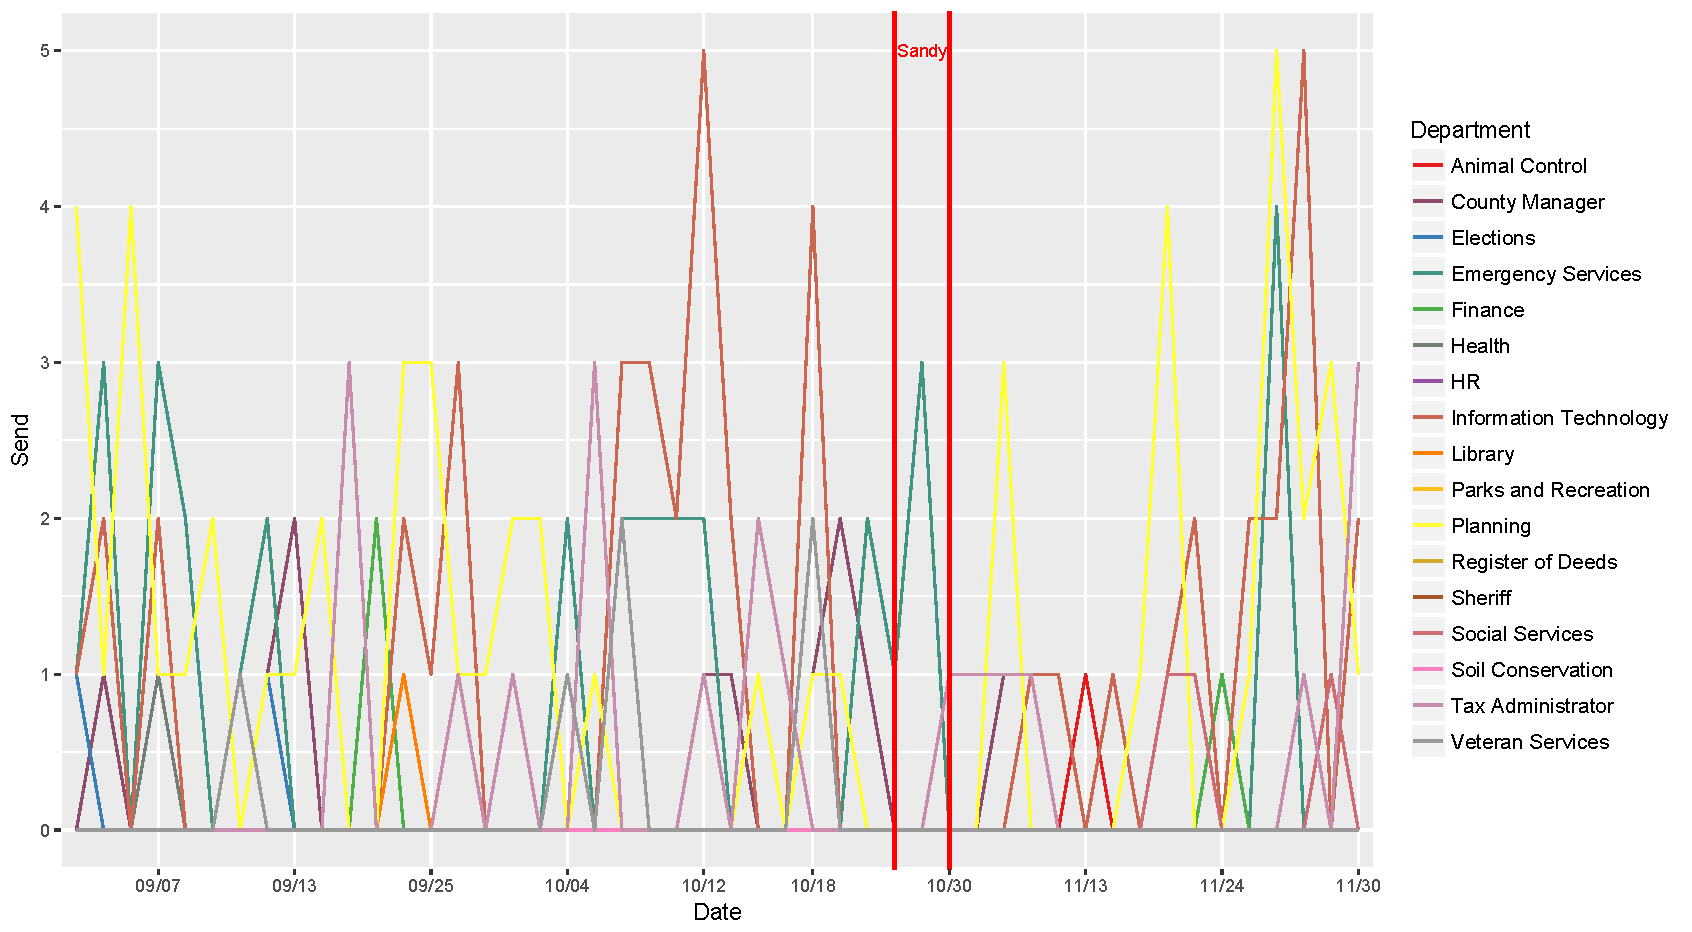
\includegraphics[width=0.5\textwidth, trim = 0cm 0cm 5cm 0cm, clip=true]{figures/VanceSend.pdf}	 	
	 	 	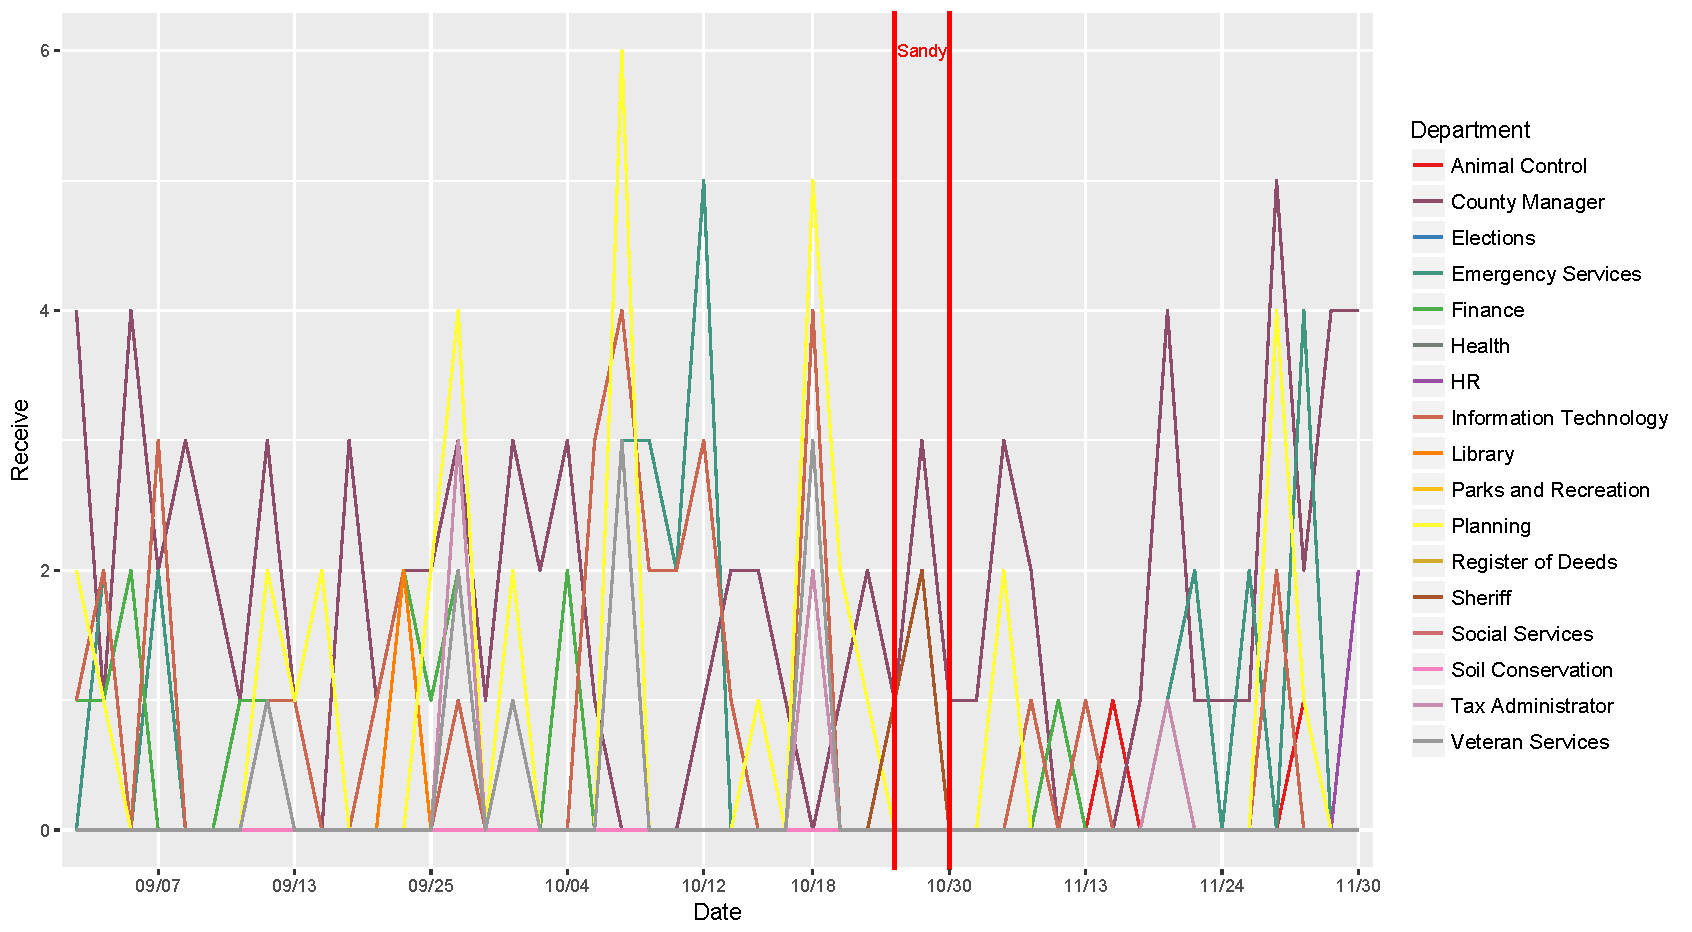
\includegraphics[width=0.5\textwidth, trim = 0cm 0cm 5cm 0cm, clip=true]{figures/VanceReceive.pdf}
	 	 \end{figure}	\vspace{-.5cm}
	 \begin{figure}
	 %	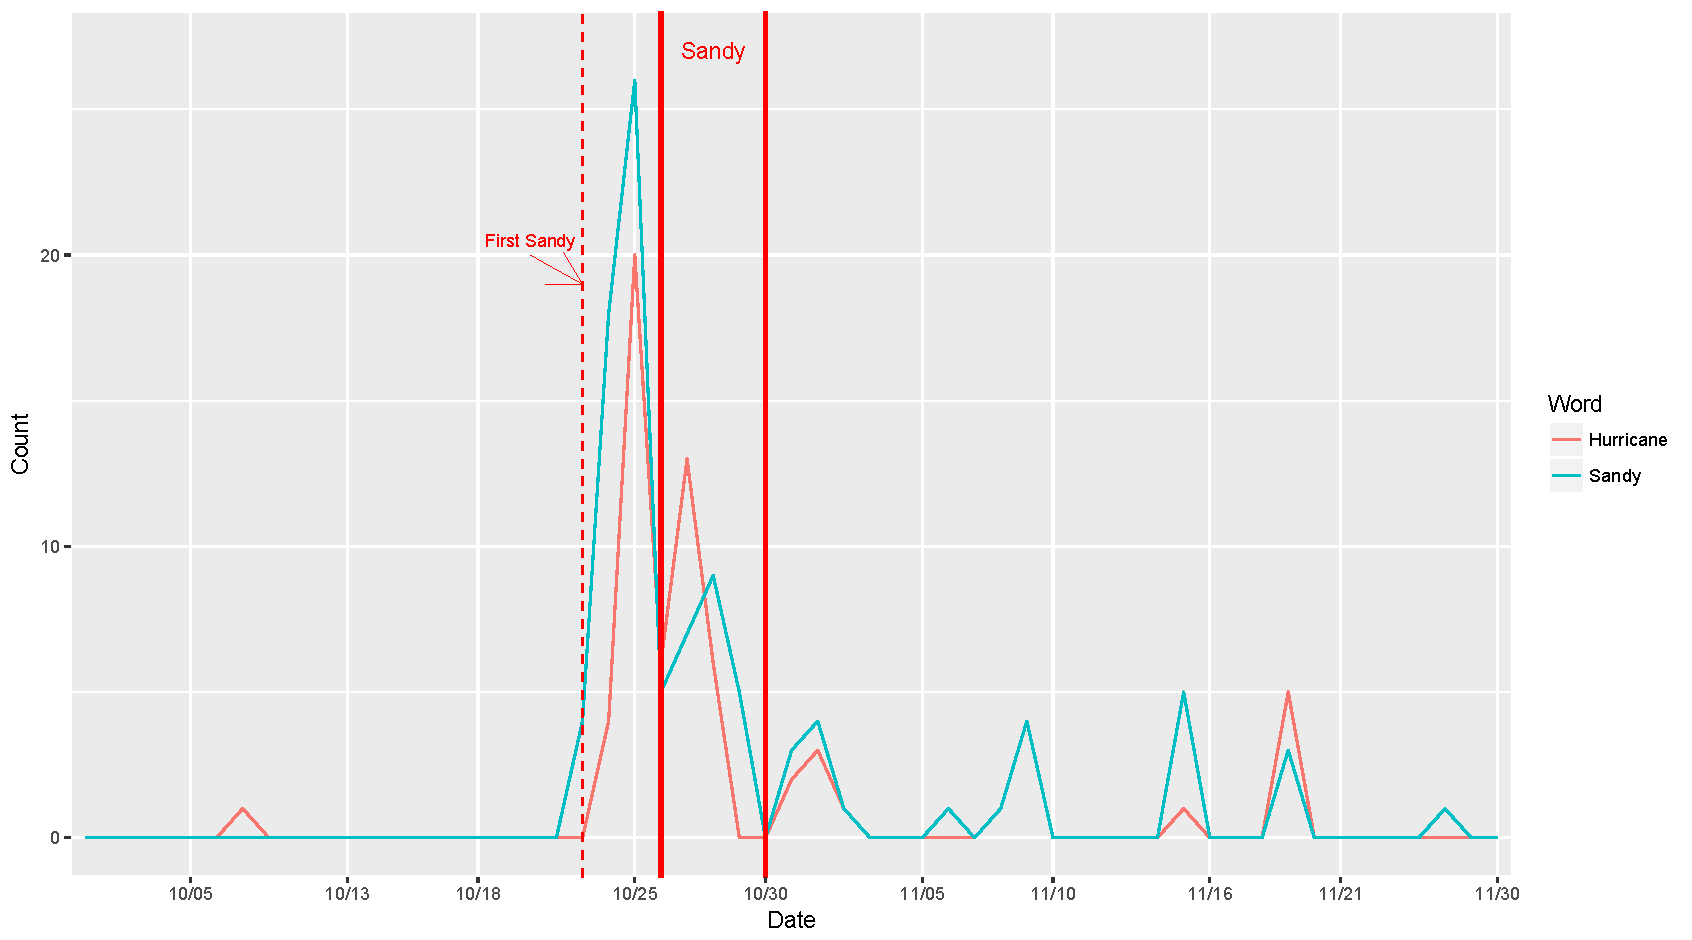
\includegraphics[width=0.5\textwidth]{Wordplot.pdf}	 
	 		 	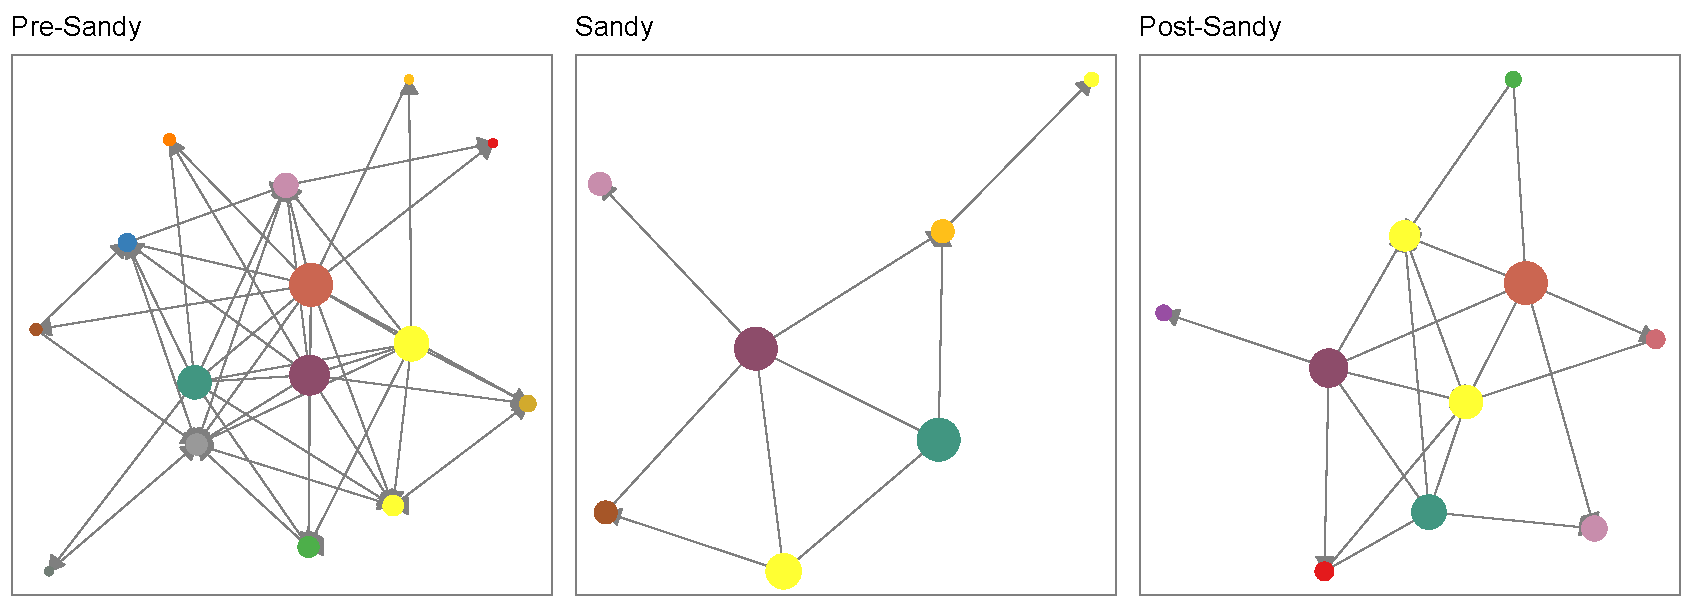
\includegraphics[width=1\textwidth]{figures/VanceNetwork.pdf}
	 		 		 \end{figure}	
\end{minipage} 
\begin{minipage}{0.13\linewidth}
		 \begin{figure}
	 		 		 	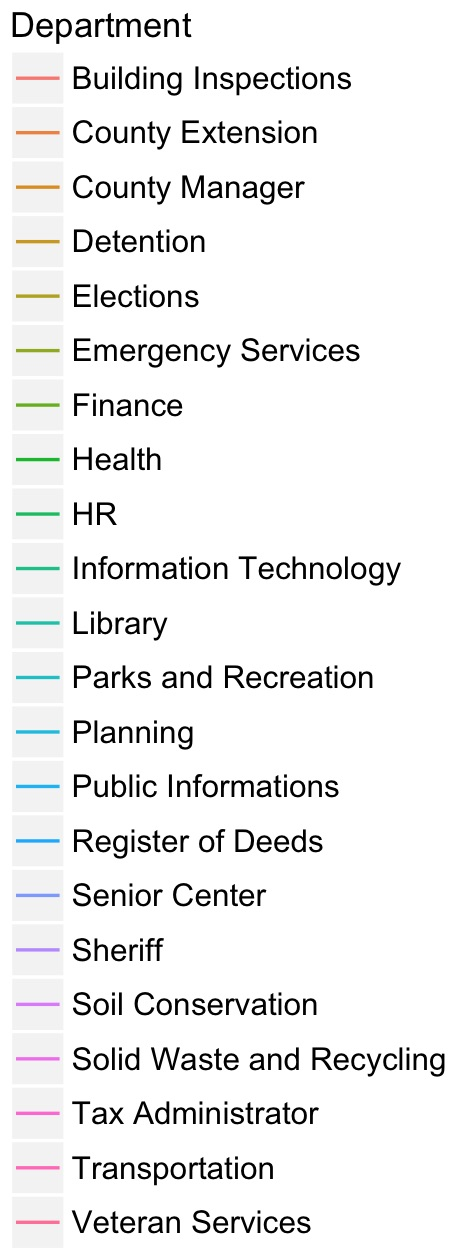
\includegraphics[width=1.25\textwidth]{figures/Dept2.jpg}
	 \end{figure}	
	\end{minipage}
\end{frame}


\begin{frame}{Exploratory Data Analysis: Dare County}
	\begin{minipage}{0.85\linewidth}
	 	 \begin{figure}
	 	 	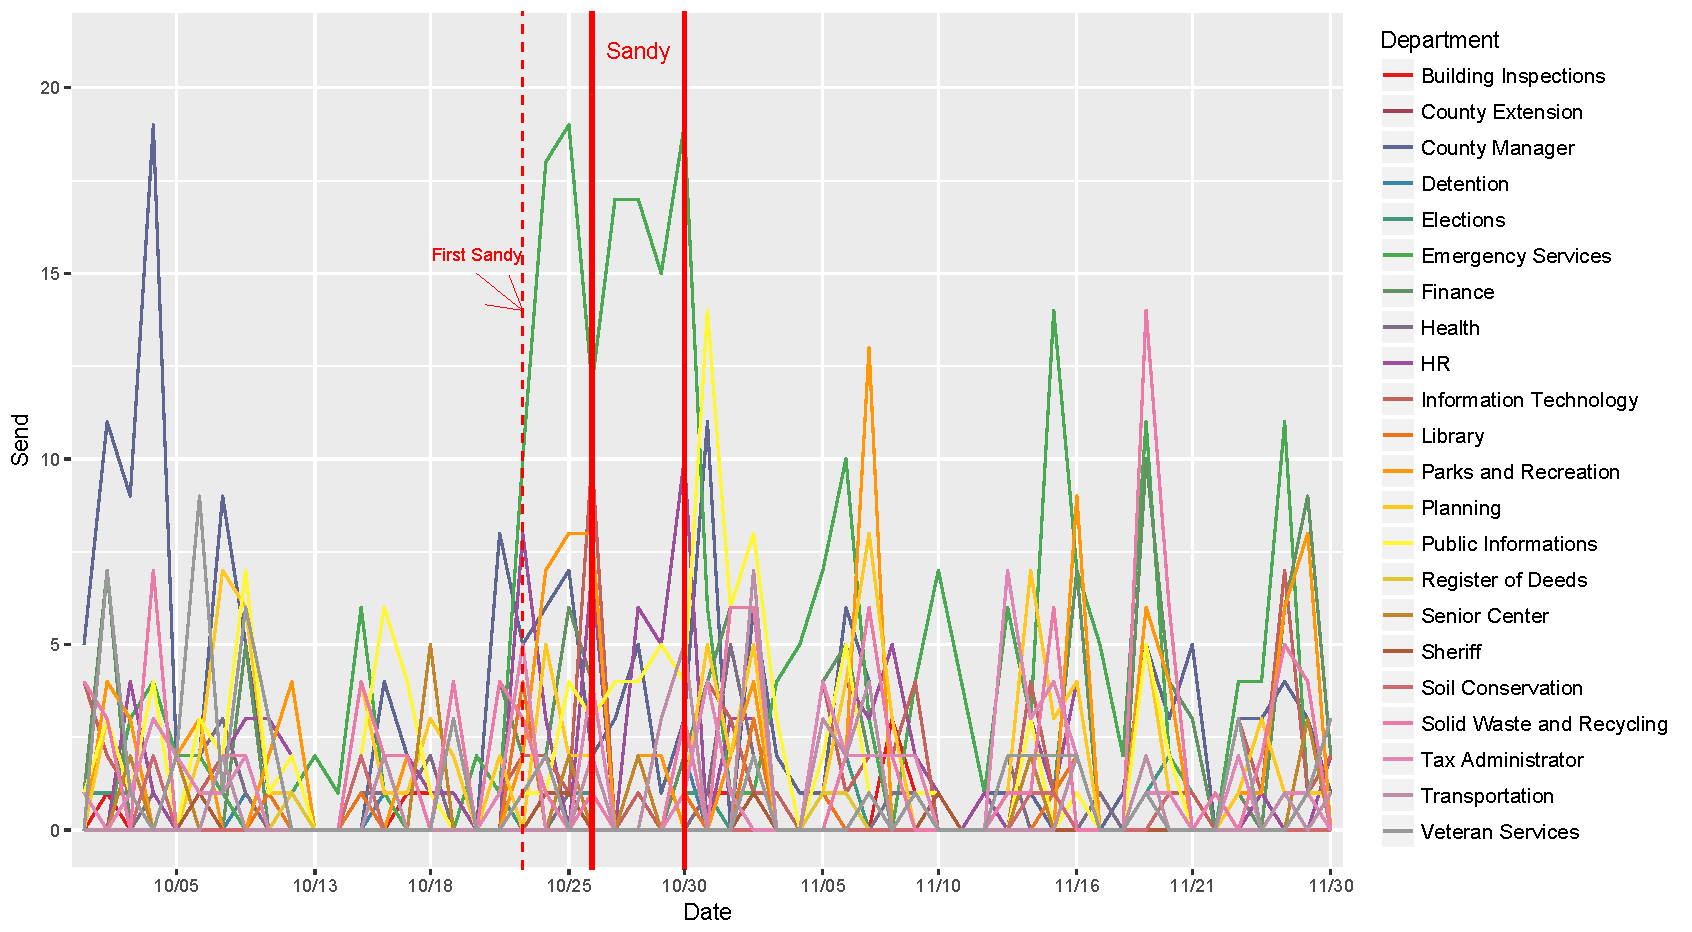
\includegraphics[width=0.5\textwidth, trim = 0cm 0cm 5cm 0cm, clip=true]{figures/DareSend.pdf}	 	
	 	 	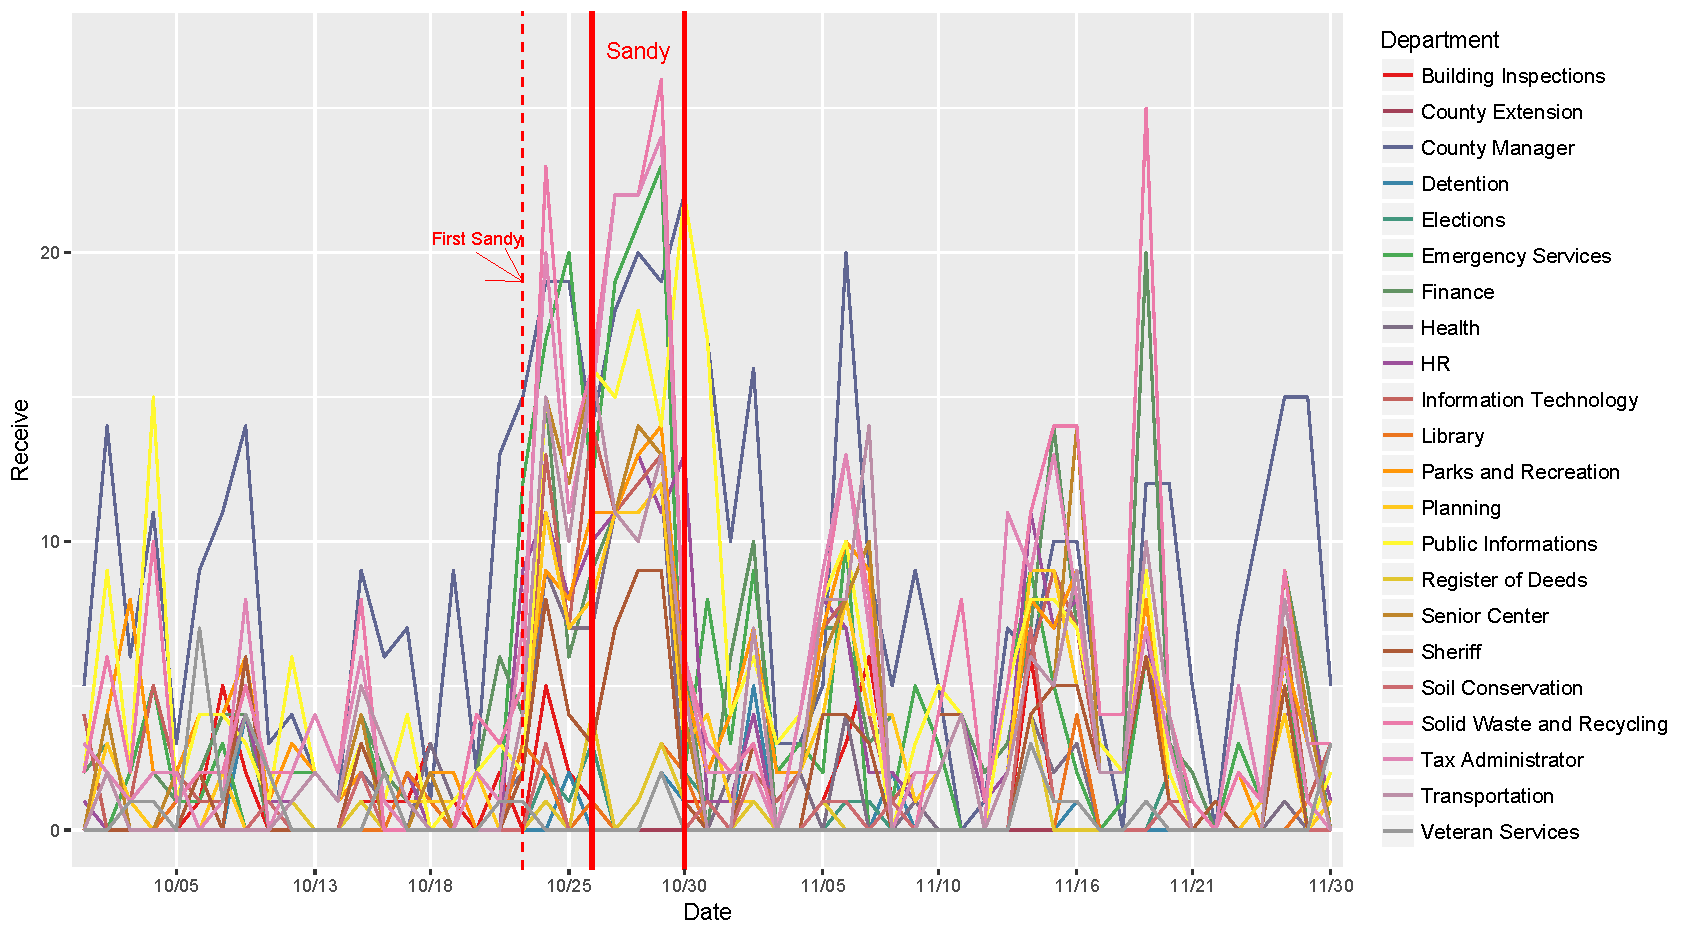
\includegraphics[width=0.5\textwidth, trim = 0cm 0cm 5cm 0cm, clip=true]{figures/DareReceive.pdf}
	 	 \end{figure}	\vspace{-.5cm}
	 \begin{figure}
	 %	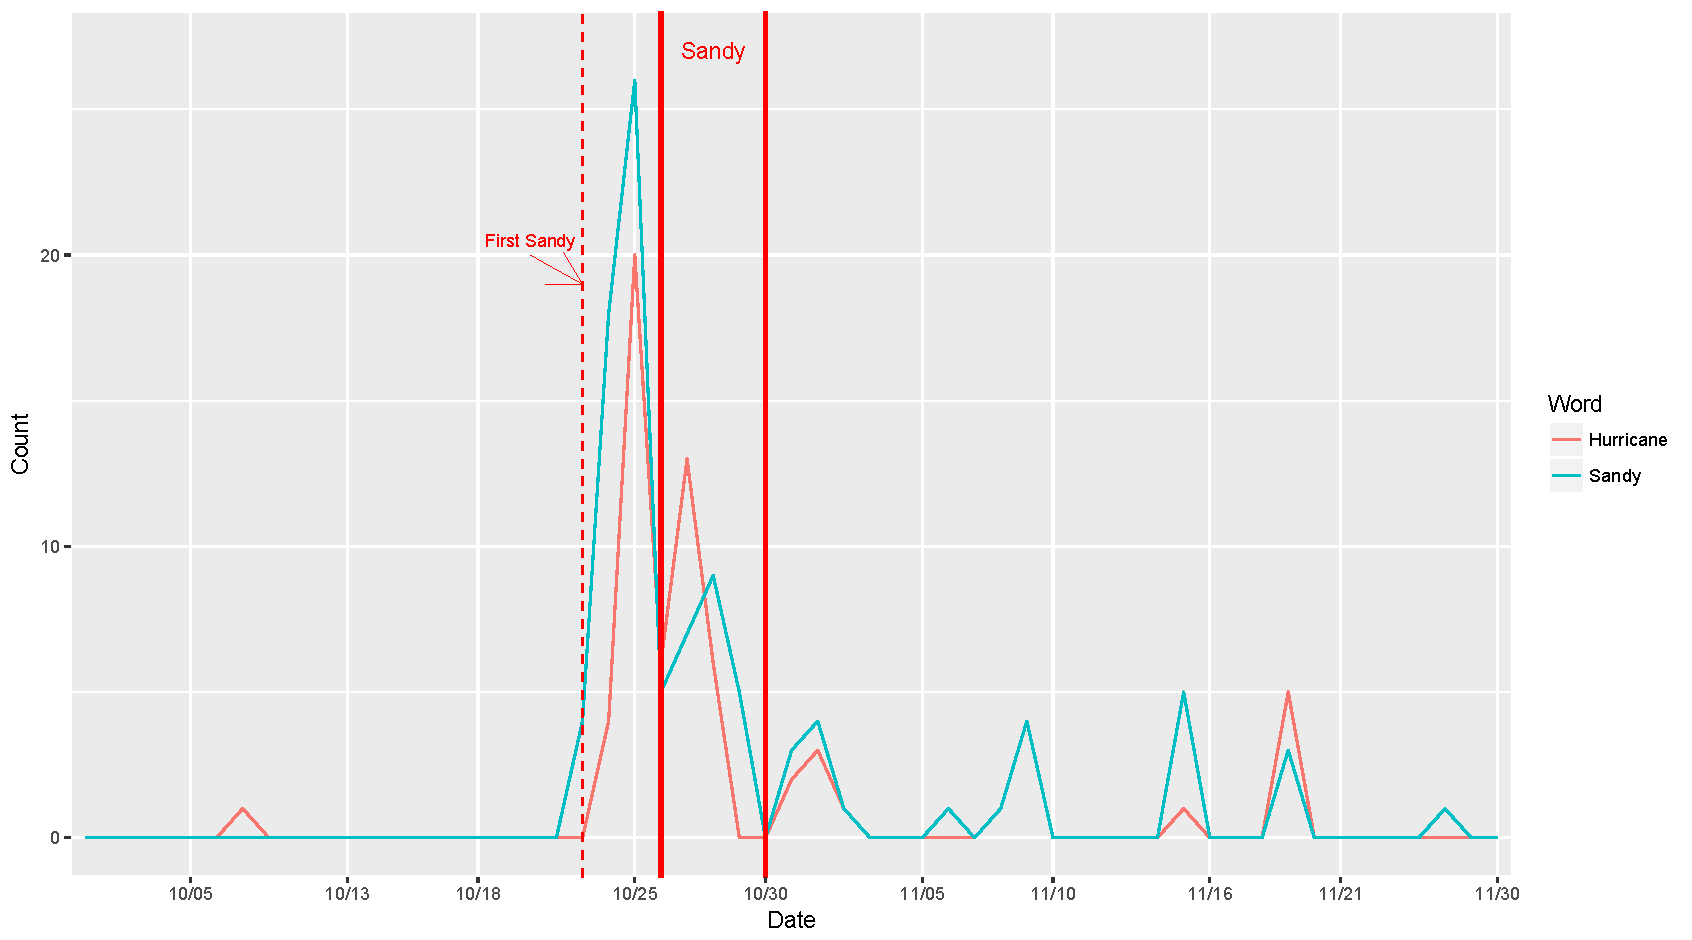
\includegraphics[width=0.5\textwidth]{Wordplot.pdf}	 
	 		 	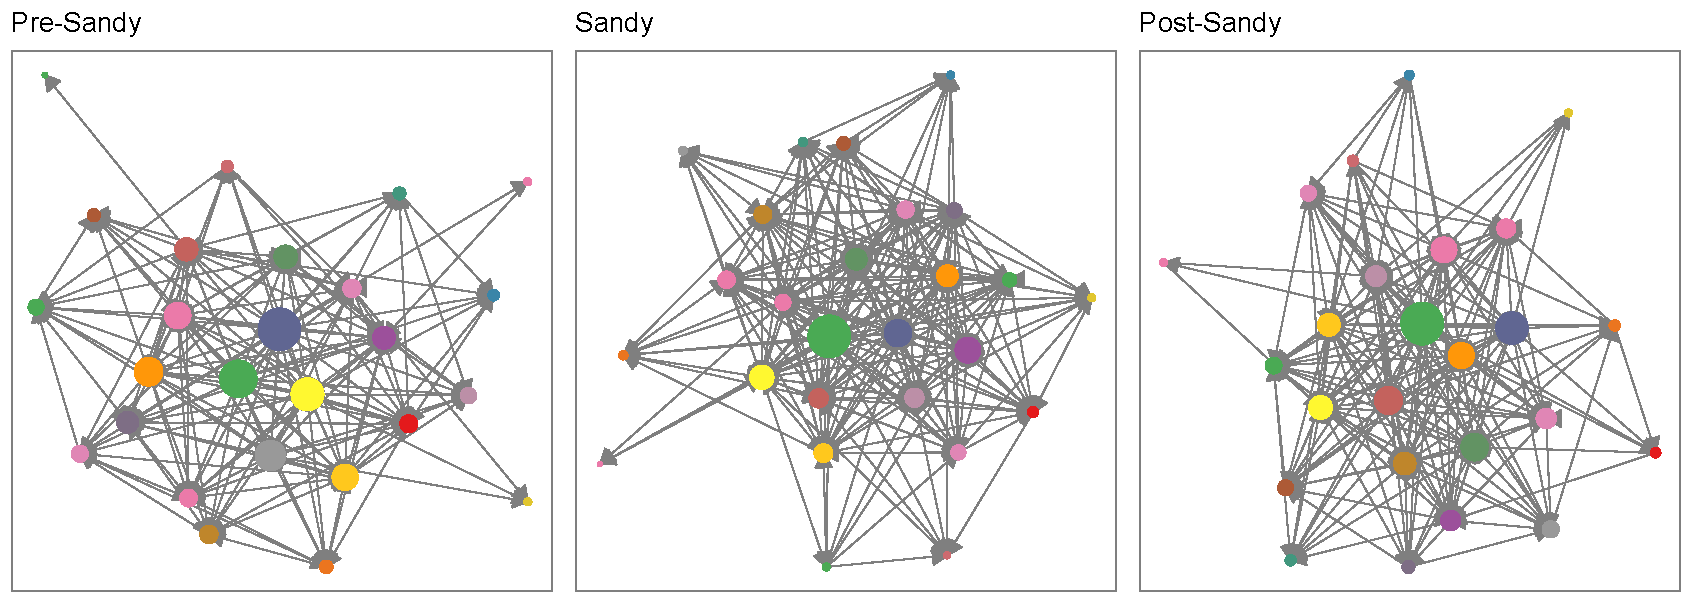
\includegraphics[width=1\textwidth]{figures/DareNetwork.pdf}
	 		 		 \end{figure}	
\end{minipage}
\begin{minipage}{0.13\linewidth}
		 \begin{figure}
	 		 		 	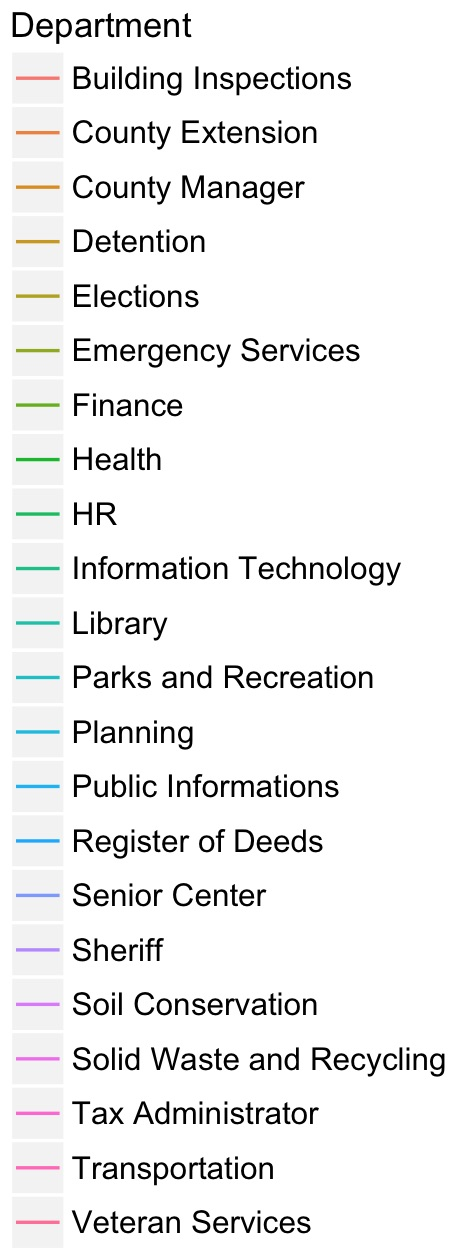
\includegraphics[width=1.25\textwidth]{figures/Dept2.jpg}
	 \end{figure}	
	\end{minipage}
\end{frame}



 \begin{frame}{IPTM Result: Topics, Vance County}
 	  $C=2$, $K=20$ and $O= 500$
 
               	\centering
               	\scalebox{0.75}{	 	\begin{tabular}{ |c||c|c|c||c|c|c|} 
               			\hline
               			\textbf{IP} & \textbf{1} &  \textbf{1} & \textbf{1}  &\textbf{2} &\textbf{2}  &\textbf{2}  \\ \hline\hline
               			\textbf{Topic} & \textbf{1} (0.078)&  \textbf{3} (0.224)& \textbf{5} (0.141) &\textbf{2} (0.139) &\textbf{4} (0.369) &\textbf{6} (0.038) \\ \hline\hline
               			\textbf{Word}
               			& directory & message & operations& phase& dropbox & phones\\
               			&switch & electronic & emergency& description & cecd & october\\
               			&network & ncgs & office &planning & henderson-vance & will\\
               			&address &  chapter  &  communications&board& box& polycom\\
               			&extension & response  & center& water & commission & intstructions\\
               			&tax & public &lines &taps& economic & training\\
               			&latest& manager & fax& keep & unemployment&conference\\
               			&department & attachments &enp & phone& licensed & three\\
               			&henderson&  siemens&cem & compliance& rural& finalized\\
               			&january & pursuant & suite&  signups & development &room\\
               			&young & subject & good&meter & reduced&cutover\\
               			&wireless & review& asap& suite & financial& contact\\
               			&installation & records& henderson&fax & private& thursday\\
               			&cutting&jail & street &meeting& labor& folks\\
               			&rest& hereto & church & tuesday& force& finishing\\
               			\hline
               		\end{tabular}}
\end{frame}


\begin{frame}{IPTM Result: Dynamic Network Effects}
	\bni \item IPTM result with $C=2$, $K=20$ and $O= 20$\footnote{Preliminary results with small outer iterations. Model results subject to change.}:
	\ei
	\begin{figure}
		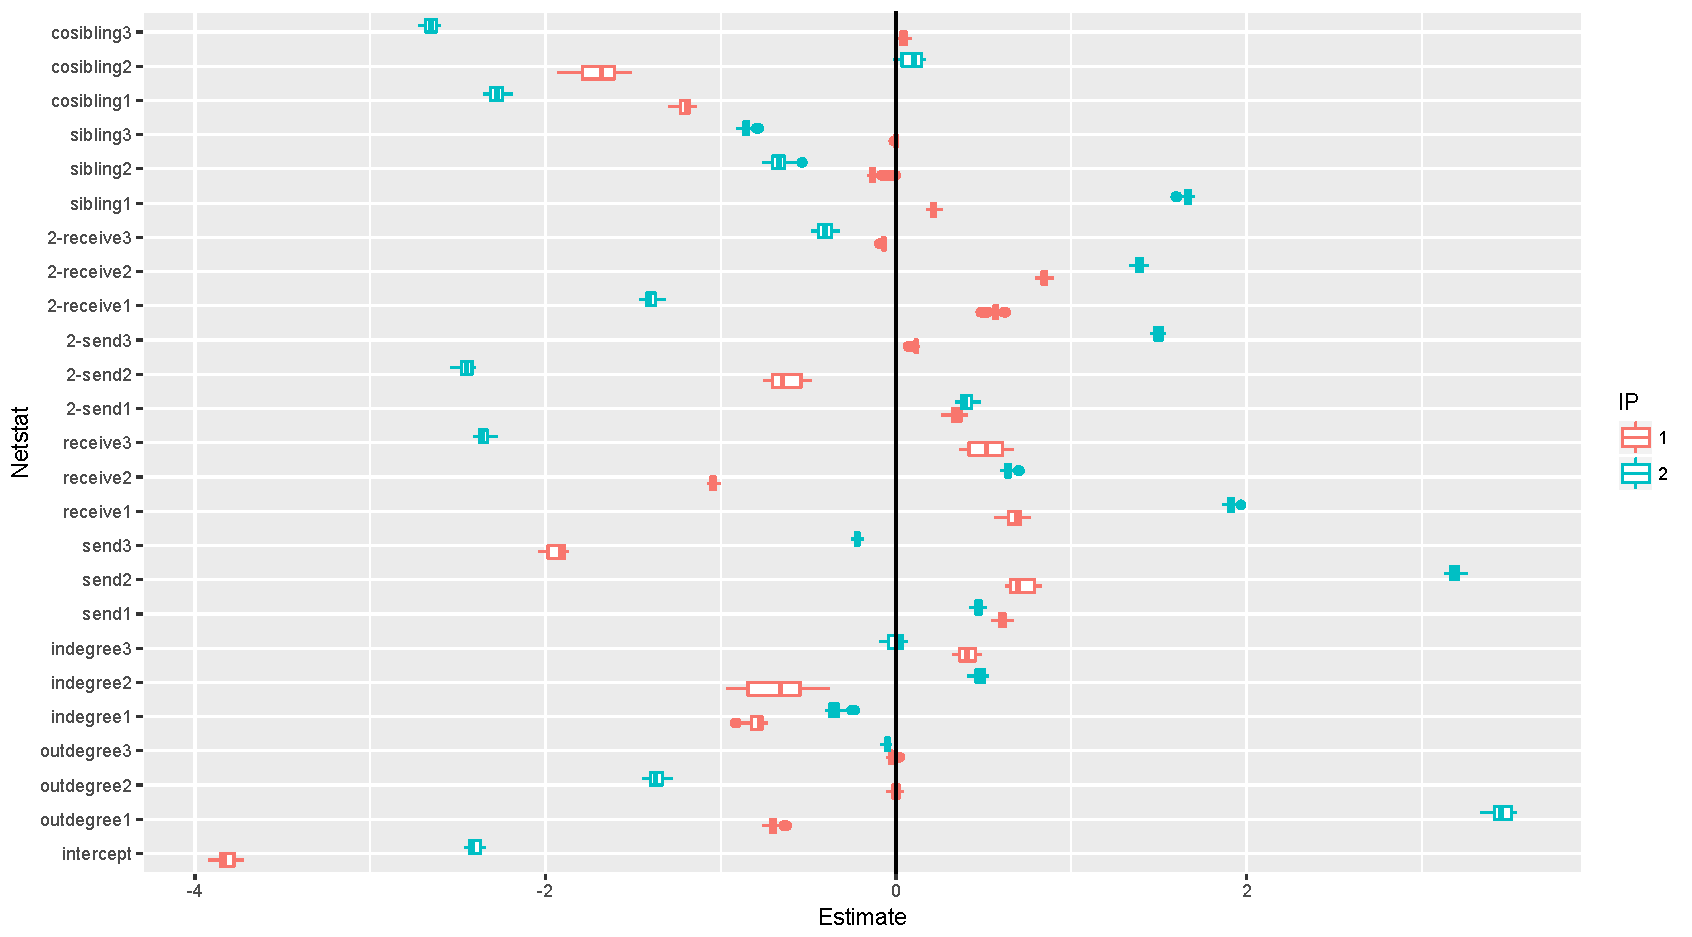
\includegraphics[width=1\textwidth]{figures/DareBplot2.pdf}
	\end{figure}	
\end{frame}


 \begin{frame}{IPTM Result: Topics, Dare County (IP 1)}
 \centering
 	 $C=2$, $K=20$ and $O= 100$
          			\scalebox{0.85}{	 	\begin{tabular}{ |c||c|c|c|c|c|}  
          					\hline
          					\textbf{IP} & \textbf{1} &  \textbf{1} & \textbf{1}  &\textbf{1} &\textbf{1}   \\ \hline\hline
          					\textbf{Topic} & \textbf{3} (0.078)&  \textbf{5} (0.065)& \textbf{19} (0.064) &\textbf{13} (0.057) &\textbf{15} (0.053)  \\ \hline\hline
          					\textbf{Word} 
          					& water & planning &phone &questions &contact\\
          					& relocation & meter & collins & board & info \\
          					& location & room & drive &december & problem\\
          					& hills& asked &marshall & call & release \\
          					& utilities &needed & director & sheets & check \\
          					& mustian & sure & human & agenda & weather \\
          					& hydrant &afternoon &resources & nov & priority \\
          					& department &cheryl & manteo & hope & readings \\
          					& skyco & johnson & phr & item & rodanthe \\
          					& kill & issues & fax & weekly & top \\
          					& devil & case & box & management & collection\\ 
          					& road & letter & timesheets &internet & located \\
          					& lane & antennas & -lsb- & told & health \\
          					& tank & inspection & wanted & care & heads \\
          					& map & keep & touch & comp & ahead\\
          					\hline       				
          				\end{tabular}}
\end{frame}


\begin{frame}{IPTM Result: Topics, Dare County (IP 2)}
 \centering
 	 $C=2$, $K=20$ and $O= 100$
          			\scalebox{0.85}{	 	\begin{tabular}{ |c||c|c|c|c|c|}  
          					\hline
          			          					\textbf{IP} & \textbf{2} &  \textbf{2} & \textbf{2}  &\textbf{2} &\textbf{2}   \\ \hline\hline
          					\textbf{Topic} & \textbf{14} (0.058)&  \textbf{12} (0.047)& \textbf{2} (0.045) &\textbf{6} (0.044) &\textbf{18} (0.036) \\ \hline\hline
          					\textbf{Word}
          					& time & survey &  road & library & status \\
          					& hours & voice & mirlo & week & system \\
          					& leave & copy& storm &  working & area \\
          					& monday & discovery & beach & place & south \\
          					& administrative & regional & high & best & forecast \\
          					& employees & parties & coastal & start & track \\
          					& empoyee & disclosed & impacts & visit & pay \\
          					& work & elections & saturday & year & move \\
          					& day & pin & dot & albemarle & assessment \\
          					& friday & sending & night & librarian & opens \\
          					& october & prior & winds & web & damage\\
          					& storm &editor & hold & learning & well\\
          					& tomorrow & students & bridge & east& ocean\\
          					& hour & cost & expressed & holiday &  operation\\
          					& question & residents & normal & system & addition
          					\\
          					\hline            				
          				\end{tabular}}
\end{frame}



\begin{frame}{IPTM Result: Dynamic Network Effects DARE}
	\bni \item IPTM result with $C=2$, $K=20$ and $O= 20$\footnote{Preliminary results with small outer iterations. Model results subject to change.}:
	\ei
	\begin{figure}
		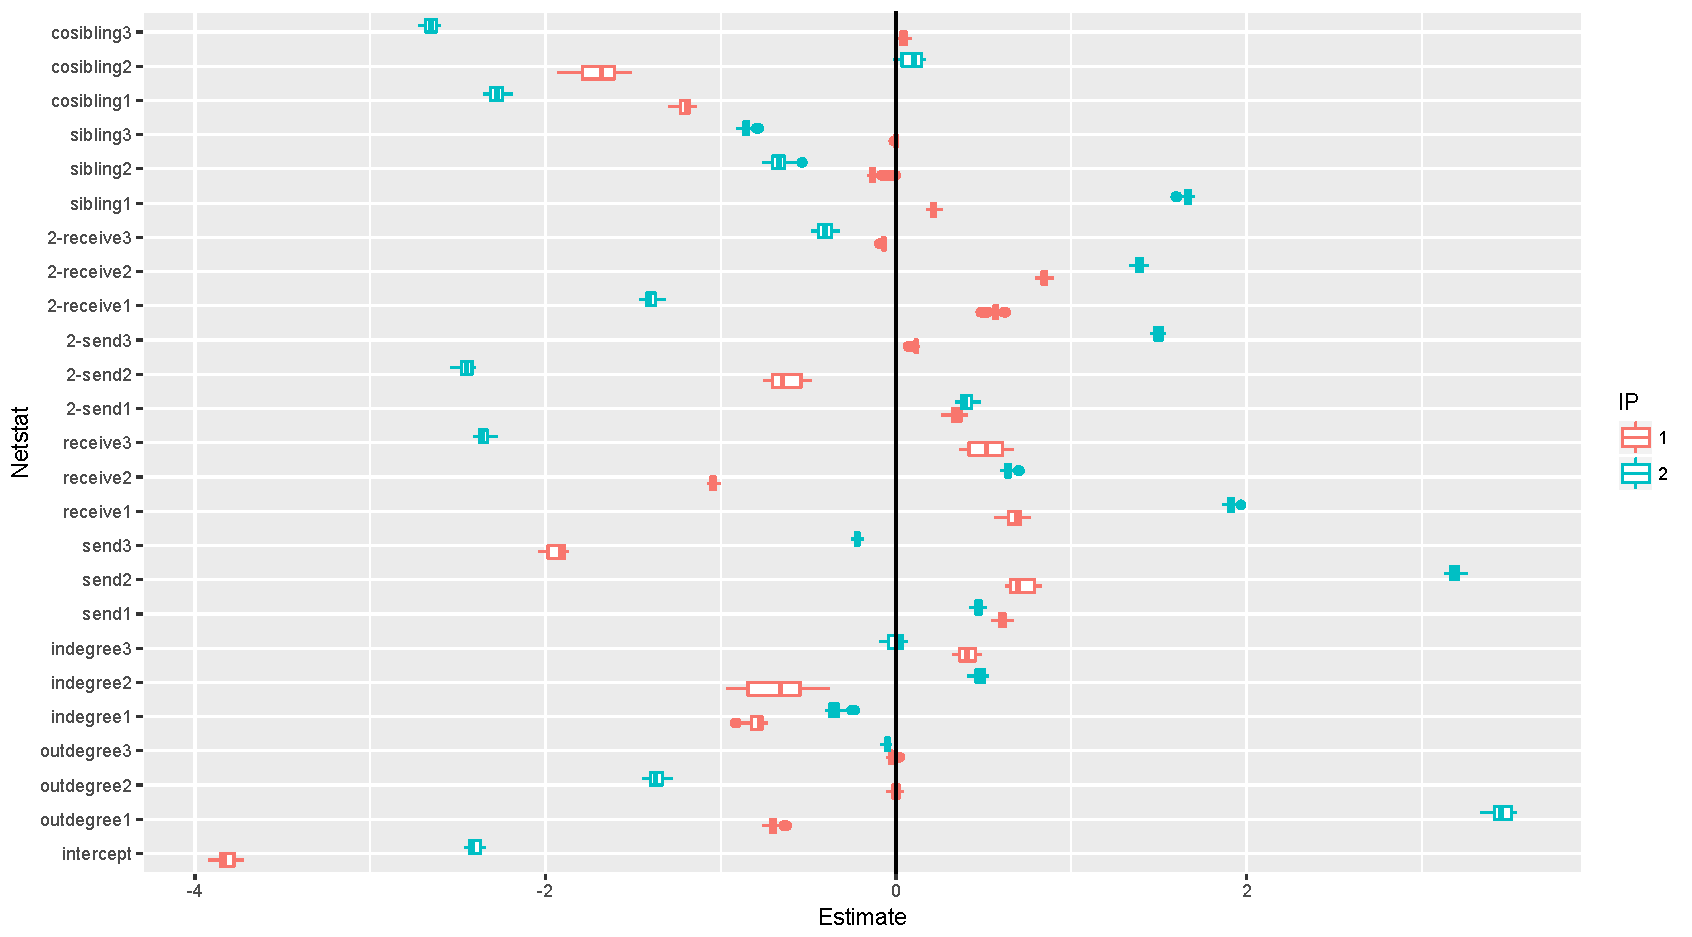
\includegraphics[width=1\textwidth]{figures/DareBplot2.pdf}
	\end{figure}	
\end{frame}


\begin{frame} \frametitle{Model fit evaluation}
\begin{itemize}
\item Forecast topics, ties, and timing of next document
\item Compare to one or more models that can generate same predictions
\end{itemize}
\scalebox{.8}{
 \begin{minipage}{1\linewidth}\begin{algorithm}[H]
	\SetAlgoLined
	\caption{Predicting tie data for the next document}
	
	Input
	\begin{enumerate}
	\item $O$, number of outer iterations of inference from which to generate predictions
	\item $d$, the last document to use in inference
	\item $R$, the number of iterations to sample predicted data within each outer iteration
	\end{enumerate}
	Run burnin iterations\\
	\For{o=1 to O}{
		run an outer iteration of inference on documents $1$ through $d$\\
		initialize values for $i^{(d+1)}$, $J^{(d+1)}$, $t^{(d+1)}$, and $\mathcal{Z}^{d+1}$ \\
		\For{r=1 to R}{
		sample  $i^{(d+1)}$, $J^{(d+1)}$, and $t^{(d+1)}$ conditional on $\mathcal{Z}^{d+1}$, via the generative process \\
		sample $\mathcal{Z}^{d+1}$ via Equation 24
		}
		store $i^{(d+1)}$, $J^{(d+1)}$, $t^{(d+1)}$, and $\mathcal{Z}^{d+1}$
	}
\end{algorithm}
\end{minipage}
}

\end{frame}


\begin{frame}{Conclusion}
 \bni
 \item Joint modeling of ties (sender, receiver, time) and contents
 	\vspace{0.4cm}
 \item Allowance of multicast -- single sender and multiple receivers
 	\vspace{0.4cm}
 \item Possible application to various political science data
 	\vspace{0.4cm}
 	\item Developement of R package `IPTM'
 \ei
\end{frame}



\begin{frame} \frametitle{Convergence of Markov Chains}



\end{frame}

\end{document}